% Options for packages loaded elsewhere
\PassOptionsToPackage{unicode}{hyperref}
\PassOptionsToPackage{hyphens}{url}
%
\documentclass[
]{article}
\usepackage{amsmath,amssymb}
\usepackage{lmodern}
\usepackage{iftex}
\ifPDFTeX
  \usepackage[T1]{fontenc}
  \usepackage[utf8]{inputenc}
  \usepackage{textcomp} % provide euro and other symbols
\else % if luatex or xetex
  \usepackage{unicode-math}
  \defaultfontfeatures{Scale=MatchLowercase}
  \defaultfontfeatures[\rmfamily]{Ligatures=TeX,Scale=1}
\fi
% Use upquote if available, for straight quotes in verbatim environments
\IfFileExists{upquote.sty}{\usepackage{upquote}}{}
\IfFileExists{microtype.sty}{% use microtype if available
  \usepackage[]{microtype}
  \UseMicrotypeSet[protrusion]{basicmath} % disable protrusion for tt fonts
}{}
\makeatletter
\@ifundefined{KOMAClassName}{% if non-KOMA class
  \IfFileExists{parskip.sty}{%
    \usepackage{parskip}
  }{% else
    \setlength{\parindent}{0pt}
    \setlength{\parskip}{6pt plus 2pt minus 1pt}}
}{% if KOMA class
  \KOMAoptions{parskip=half}}
\makeatother
\usepackage{xcolor}
\usepackage[margin=1in]{geometry}
\usepackage{color}
\usepackage{fancyvrb}
\newcommand{\VerbBar}{|}
\newcommand{\VERB}{\Verb[commandchars=\\\{\}]}
\DefineVerbatimEnvironment{Highlighting}{Verbatim}{commandchars=\\\{\}}
% Add ',fontsize=\small' for more characters per line
\usepackage{framed}
\definecolor{shadecolor}{RGB}{248,248,248}
\newenvironment{Shaded}{\begin{snugshade}}{\end{snugshade}}
\newcommand{\AlertTok}[1]{\textcolor[rgb]{0.94,0.16,0.16}{#1}}
\newcommand{\AnnotationTok}[1]{\textcolor[rgb]{0.56,0.35,0.01}{\textbf{\textit{#1}}}}
\newcommand{\AttributeTok}[1]{\textcolor[rgb]{0.77,0.63,0.00}{#1}}
\newcommand{\BaseNTok}[1]{\textcolor[rgb]{0.00,0.00,0.81}{#1}}
\newcommand{\BuiltInTok}[1]{#1}
\newcommand{\CharTok}[1]{\textcolor[rgb]{0.31,0.60,0.02}{#1}}
\newcommand{\CommentTok}[1]{\textcolor[rgb]{0.56,0.35,0.01}{\textit{#1}}}
\newcommand{\CommentVarTok}[1]{\textcolor[rgb]{0.56,0.35,0.01}{\textbf{\textit{#1}}}}
\newcommand{\ConstantTok}[1]{\textcolor[rgb]{0.00,0.00,0.00}{#1}}
\newcommand{\ControlFlowTok}[1]{\textcolor[rgb]{0.13,0.29,0.53}{\textbf{#1}}}
\newcommand{\DataTypeTok}[1]{\textcolor[rgb]{0.13,0.29,0.53}{#1}}
\newcommand{\DecValTok}[1]{\textcolor[rgb]{0.00,0.00,0.81}{#1}}
\newcommand{\DocumentationTok}[1]{\textcolor[rgb]{0.56,0.35,0.01}{\textbf{\textit{#1}}}}
\newcommand{\ErrorTok}[1]{\textcolor[rgb]{0.64,0.00,0.00}{\textbf{#1}}}
\newcommand{\ExtensionTok}[1]{#1}
\newcommand{\FloatTok}[1]{\textcolor[rgb]{0.00,0.00,0.81}{#1}}
\newcommand{\FunctionTok}[1]{\textcolor[rgb]{0.00,0.00,0.00}{#1}}
\newcommand{\ImportTok}[1]{#1}
\newcommand{\InformationTok}[1]{\textcolor[rgb]{0.56,0.35,0.01}{\textbf{\textit{#1}}}}
\newcommand{\KeywordTok}[1]{\textcolor[rgb]{0.13,0.29,0.53}{\textbf{#1}}}
\newcommand{\NormalTok}[1]{#1}
\newcommand{\OperatorTok}[1]{\textcolor[rgb]{0.81,0.36,0.00}{\textbf{#1}}}
\newcommand{\OtherTok}[1]{\textcolor[rgb]{0.56,0.35,0.01}{#1}}
\newcommand{\PreprocessorTok}[1]{\textcolor[rgb]{0.56,0.35,0.01}{\textit{#1}}}
\newcommand{\RegionMarkerTok}[1]{#1}
\newcommand{\SpecialCharTok}[1]{\textcolor[rgb]{0.00,0.00,0.00}{#1}}
\newcommand{\SpecialStringTok}[1]{\textcolor[rgb]{0.31,0.60,0.02}{#1}}
\newcommand{\StringTok}[1]{\textcolor[rgb]{0.31,0.60,0.02}{#1}}
\newcommand{\VariableTok}[1]{\textcolor[rgb]{0.00,0.00,0.00}{#1}}
\newcommand{\VerbatimStringTok}[1]{\textcolor[rgb]{0.31,0.60,0.02}{#1}}
\newcommand{\WarningTok}[1]{\textcolor[rgb]{0.56,0.35,0.01}{\textbf{\textit{#1}}}}
\usepackage{graphicx}
\makeatletter
\def\maxwidth{\ifdim\Gin@nat@width>\linewidth\linewidth\else\Gin@nat@width\fi}
\def\maxheight{\ifdim\Gin@nat@height>\textheight\textheight\else\Gin@nat@height\fi}
\makeatother
% Scale images if necessary, so that they will not overflow the page
% margins by default, and it is still possible to overwrite the defaults
% using explicit options in \includegraphics[width, height, ...]{}
\setkeys{Gin}{width=\maxwidth,height=\maxheight,keepaspectratio}
% Set default figure placement to htbp
\makeatletter
\def\fps@figure{htbp}
\makeatother
\setlength{\emergencystretch}{3em} % prevent overfull lines
\providecommand{\tightlist}{%
  \setlength{\itemsep}{0pt}\setlength{\parskip}{0pt}}
\setcounter{secnumdepth}{-\maxdimen} % remove section numbering
\ifLuaTeX
  \usepackage{selnolig}  % disable illegal ligatures
\fi
\IfFileExists{bookmark.sty}{\usepackage{bookmark}}{\usepackage{hyperref}}
\IfFileExists{xurl.sty}{\usepackage{xurl}}{} % add URL line breaks if available
\urlstyle{same} % disable monospaced font for URLs
\hypersetup{
  pdftitle={Quiz 4},
  pdfauthor={Eduardo Armenta},
  hidelinks,
  pdfcreator={LaTeX via pandoc}}

\title{Quiz 4}
\author{Eduardo Armenta}
\date{2022-10-28}

\begin{document}
\maketitle

\hypertarget{quiz-4}{%
\section{Quiz 4}\label{quiz-4}}

\hypertarget{problem-1}{%
\subsection{Problem 1}\label{problem-1}}

Here is an image of the first problem.

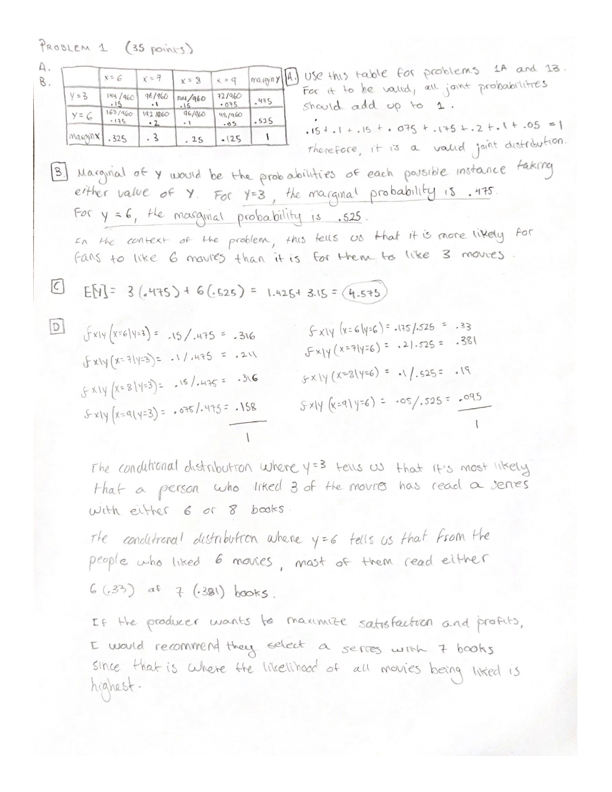
\includegraphics{./Q1.png}

\hypertarget{problem-2}{%
\subsection{Problem 2}\label{problem-2}}

These are the answers to the first three parts of problem 2.

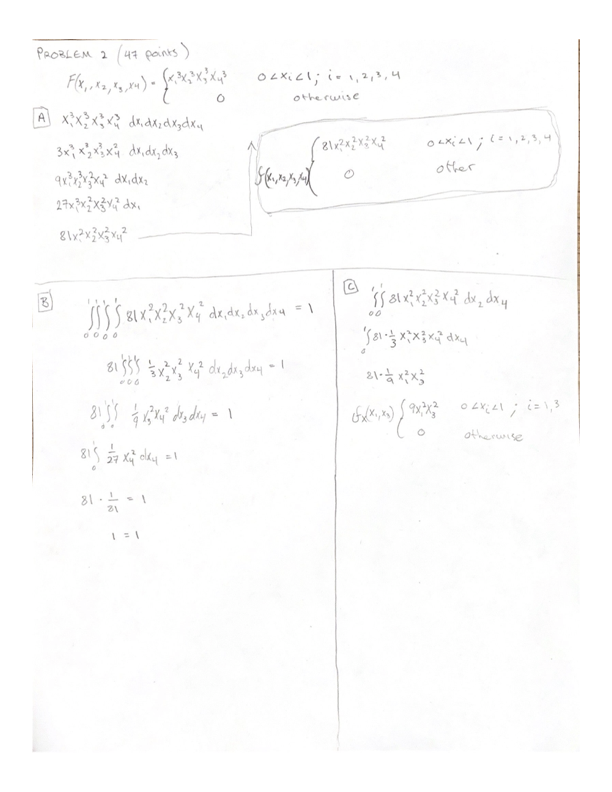
\includegraphics{./Q2sideA.png}

These are the answers to the last 2 parts of problem 2.

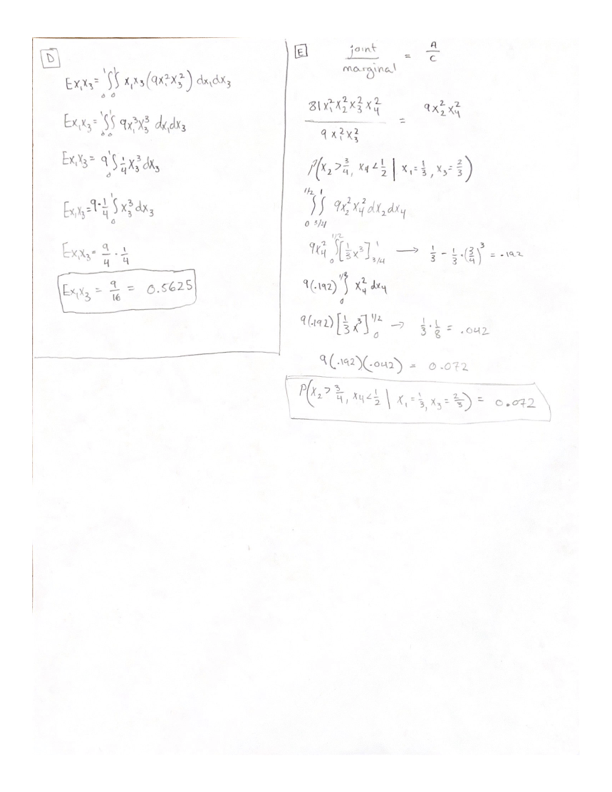
\includegraphics{./Q2sideB.png}

\hypertarget{problem-3}{%
\subsection{Problem 3}\label{problem-3}}

\textbf{a.} (10 points) Describe your game and describe how it is a
Markov process. (Hint: Remember the game rules will help you to make
sure it is a Markov process)

We are playing on a one-dimensional, horizontal board with 7 tiles that
are lettered A trough G in alphabetical order. The goal is to reach
letter G. In order to advance through the board, we must throw a
six-sided die. The die roll will ask you to move in the following
manner:

\begin{itemize}
\tightlist
\item
  1: Move forward one letter
\item
  2: Move backward one letter
\item
  3: Move forward two letters
\item
  4: Move back to A
\item
  5: Don't move
\item
  6: Go straight to G
\end{itemize}

You cannot go further back than A. That is, if you roll a 2 while at A,
you will remain at A. In order to land at G from F, you have to roll a 6
or a 1, you can't land on G by rolling a 3 (unless you're at E). Once
you get to G, the game is over, so the probability of leaving G is 0.

This game is a Markov Chain because each roll of the die is an
independent roll. The probability of entering another stage is not
influenced by which stage you're in or which number you got in the
previous roll.

\textbf{b.} (10 points) Draw the transition diagram.

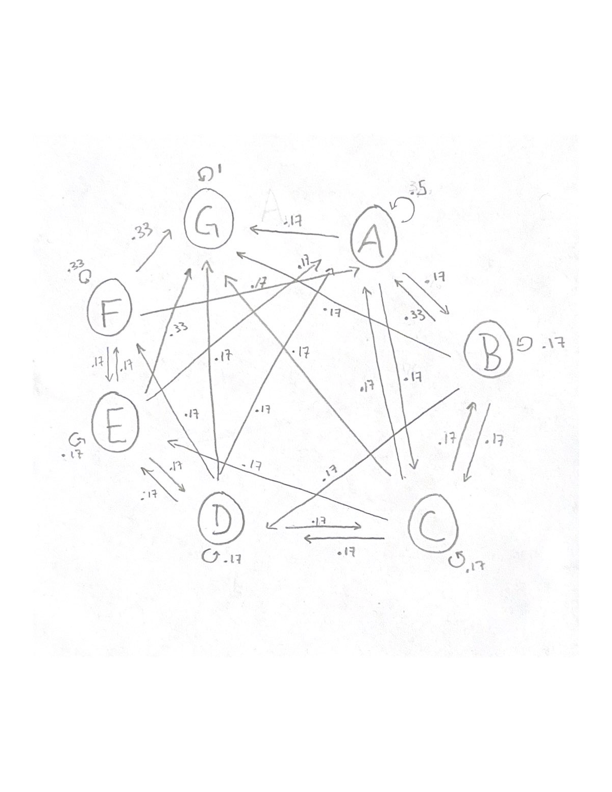
\includegraphics{./diagram.png}

\textbf{c.} (10 points) Construct the transition probability matrix.

\begin{Shaded}
\begin{Highlighting}[]
\NormalTok{probs }\OtherTok{\textless{}{-}} \FunctionTok{c}\NormalTok{(}\DecValTok{1}\SpecialCharTok{/}\DecValTok{2}\NormalTok{,  }\DecValTok{1}\SpecialCharTok{/}\DecValTok{3}\NormalTok{, }\DecValTok{1}\SpecialCharTok{/}\DecValTok{6}\NormalTok{, }\DecValTok{1}\SpecialCharTok{/}\DecValTok{6}\NormalTok{, }\DecValTok{1}\SpecialCharTok{/}\DecValTok{6}\NormalTok{, }\DecValTok{1}\SpecialCharTok{/}\DecValTok{6}\NormalTok{, }\DecValTok{0}\NormalTok{,}
            \DecValTok{1}\SpecialCharTok{/}\DecValTok{6}\NormalTok{, }\DecValTok{1}\SpecialCharTok{/}\DecValTok{6}\NormalTok{, }\DecValTok{1}\SpecialCharTok{/}\DecValTok{6}\NormalTok{, }\DecValTok{0}\NormalTok{,   }\DecValTok{0}\NormalTok{,   }\DecValTok{0}\NormalTok{,   }\DecValTok{0}\NormalTok{,}
            \DecValTok{1}\SpecialCharTok{/}\DecValTok{6}\NormalTok{, }\DecValTok{1}\SpecialCharTok{/}\DecValTok{6}\NormalTok{, }\DecValTok{1}\SpecialCharTok{/}\DecValTok{6}\NormalTok{, }\DecValTok{1}\SpecialCharTok{/}\DecValTok{6}\NormalTok{, }\DecValTok{0}\NormalTok{,   }\DecValTok{0}\NormalTok{,   }\DecValTok{0}\NormalTok{,}
            \DecValTok{0}\NormalTok{,   }\DecValTok{1}\SpecialCharTok{/}\DecValTok{6}\NormalTok{, }\DecValTok{1}\SpecialCharTok{/}\DecValTok{6}\NormalTok{, }\DecValTok{1}\SpecialCharTok{/}\DecValTok{6}\NormalTok{, }\DecValTok{1}\SpecialCharTok{/}\DecValTok{6}\NormalTok{, }\DecValTok{0}\NormalTok{,   }\DecValTok{0}\NormalTok{,}
            \DecValTok{0}\NormalTok{,   }\DecValTok{0}\NormalTok{,   }\DecValTok{1}\SpecialCharTok{/}\DecValTok{6}\NormalTok{, }\DecValTok{1}\SpecialCharTok{/}\DecValTok{6}\NormalTok{, }\DecValTok{1}\SpecialCharTok{/}\DecValTok{6}\NormalTok{, }\DecValTok{1}\SpecialCharTok{/}\DecValTok{6}\NormalTok{, }\DecValTok{0}\NormalTok{,}
            \DecValTok{0}\NormalTok{,   }\DecValTok{0}\NormalTok{,   }\DecValTok{0}\NormalTok{,   }\DecValTok{1}\SpecialCharTok{/}\DecValTok{6}\NormalTok{, }\DecValTok{1}\SpecialCharTok{/}\DecValTok{6}\NormalTok{, }\DecValTok{1}\SpecialCharTok{/}\DecValTok{3}\NormalTok{, }\DecValTok{0}\NormalTok{,}
            \DecValTok{1}\SpecialCharTok{/}\DecValTok{6}\NormalTok{, }\DecValTok{1}\SpecialCharTok{/}\DecValTok{6}\NormalTok{, }\DecValTok{1}\SpecialCharTok{/}\DecValTok{6}\NormalTok{, }\DecValTok{1}\SpecialCharTok{/}\DecValTok{6}\NormalTok{, }\DecValTok{1}\SpecialCharTok{/}\DecValTok{3}\NormalTok{, }\DecValTok{1}\SpecialCharTok{/}\DecValTok{3}\NormalTok{, }\DecValTok{1}\NormalTok{)}
\NormalTok{M }\OtherTok{\textless{}{-}} \FunctionTok{matrix}\NormalTok{(probs,}\AttributeTok{nrow=}\DecValTok{7}\NormalTok{)}
\NormalTok{M}
\end{Highlighting}
\end{Shaded}

\begin{verbatim}
##           [,1]      [,2]      [,3]      [,4]      [,5]      [,6]      [,7]
## [1,] 0.5000000 0.1666667 0.1666667 0.0000000 0.0000000 0.0000000 0.1666667
## [2,] 0.3333333 0.1666667 0.1666667 0.1666667 0.0000000 0.0000000 0.1666667
## [3,] 0.1666667 0.1666667 0.1666667 0.1666667 0.1666667 0.0000000 0.1666667
## [4,] 0.1666667 0.0000000 0.1666667 0.1666667 0.1666667 0.1666667 0.1666667
## [5,] 0.1666667 0.0000000 0.0000000 0.1666667 0.1666667 0.1666667 0.3333333
## [6,] 0.1666667 0.0000000 0.0000000 0.0000000 0.1666667 0.3333333 0.3333333
## [7,] 0.0000000 0.0000000 0.0000000 0.0000000 0.0000000 0.0000000 1.0000000
\end{verbatim}

\textbf{d.} (7 points) What is the probability that if the player is
currently in state 𝑖 (you can define state 𝑖) then they would win in 12
steps. (Define where/what state the player need to be when/if they win)

\begin{Shaded}
\begin{Highlighting}[]
\FunctionTok{print}\NormalTok{(}\FunctionTok{paste0}\NormalTok{(}\StringTok{\textquotesingle{}Beginning from letter A, the probability of getting to letter G in 12 steps is: \textquotesingle{}}\NormalTok{, (M}\SpecialCharTok{\%*\%}\NormalTok{M}\SpecialCharTok{\%*\%}\NormalTok{M}\SpecialCharTok{\%*\%}\NormalTok{M}\SpecialCharTok{\%*\%}\NormalTok{M}\SpecialCharTok{\%*\%}\NormalTok{M}\SpecialCharTok{\%*\%}\NormalTok{M}\SpecialCharTok{\%*\%}\NormalTok{M}\SpecialCharTok{\%*\%}\NormalTok{M}\SpecialCharTok{\%*\%}\NormalTok{M}\SpecialCharTok{\%*\%}\NormalTok{M}\SpecialCharTok{\%*\%}\NormalTok{M)[}\DecValTok{1}\NormalTok{,}\DecValTok{7}\NormalTok{]))}
\end{Highlighting}
\end{Shaded}

\begin{verbatim}
## [1] "Beginning from letter A, the probability of getting to letter G in 12 steps is: 0.914750617031835"
\end{verbatim}

\textbf{e.} (6 points: 2 points each) Write 3 real life examples where
we use the Markov process (except Google page rank) and write 1-2
sentences explaining it. It is okay to use Google to find it but please
include reference links for each example.

\begin{enumerate}
\def\labelenumi{\arabic{enumi}.}
\item
  Weather prediction: if we want to predict whether it'll be sunny or
  rainy in summer, we can use the Markov chain. The two states are sun
  or rain and we look at past observations to find the likelihood that a
  sunny day follows a sunny and that a rainy day follows a rainy day
  (probability of changing state is 1-probability of staying in the same
  state).
\item
  Market trends: as Dr.~Gamage mentioned in class, we can predict market
  sentiment with Markov chains. We can look at weekly historical data
  (or daily, monthly, etc.) to see if the market will enter one of the
  three possible states (i.e., bull, bear, neutral). I think it would be
  safe to assume that a bull week will most likely follow a bull week,
  and we can find the likelihood of each state remaining in one state or
  switching to another.
\item
  Next word prediction: as mentioned in one of the 511 lab case studies,
  Markov chains can be used to predict the next word of a sentence. For
  example, if we have the sentences ``I like cats'', ``I like dogs'',
  and ``I hate snakes'', the model would dictate that the first word has
  a 100\% probability of being ``I''. Then the possible states following
  ``I'' would be ``like'' (0.67 probability) and ``hate'' (0.33
  probability). Finally, there would be three possible states coming
  after the second word, which would be ``dogs'', ``cats'', and
  ``snakes'', and each one would be predicted to occur with a
  probability of 0.33.
\end{enumerate}

\end{document}
